\documentclass[11pt]{article}

\usepackage[utf8]{inputenc}
\usepackage[T1]{fontenc}
\usepackage{lmodern}
\usepackage{amsmath, amssymb}
\usepackage{xcolor}
\usepackage{tcolorbox}
\usepackage{graphicx}
\usepackage{tikz}
\usepackage{float}
\usepackage{hyperref}
\usepackage{enumitem}
\usepackage{caption}
\usepackage{listings}
\usepackage[margin=1in]{geometry}

\usetikzlibrary{shapes, arrows.meta, positioning}

\hypersetup{
  colorlinks=true,
  linkcolor=blue,
  urlcolor=blue,
  citecolor=blue
}


% --- Semantic tcolorbox styles ---
\definecolor{defblue}{RGB}{41, 98, 163}
\definecolor{insightgreen}{RGB}{46, 139, 87}
\definecolor{warnorange}{RGB}{204, 119, 34}
\definecolor{recapgray}{RGB}{100, 100, 100}
\definecolor{actionviolet}{RGB}{106, 61, 154}
\definecolor{resultteal}{RGB}{0, 128, 128}

\newtcolorbox{defbox}[1][]{colback=defblue!5!white, colframe=defblue!80, fonttitle=\bfseries, #1}
\newtcolorbox{insightbox}[1][]{colback=insightgreen!5!white, colframe=insightgreen!80, fonttitle=\bfseries, #1}
\newtcolorbox{warnbox}[1][]{colback=warnorange!6!white, colframe=warnorange!80, fonttitle=\bfseries, #1}
\newtcolorbox{recapbox}[1][]{colback=recapgray!6!white, colframe=recapgray!70, fonttitle=\bfseries, #1}
\newtcolorbox{actionbox}[1][]{colback=actionviolet!5!white, colframe=actionviolet!70, fonttitle=\bfseries, #1}
\newtcolorbox{resultbox}[1][]{colback=resultteal!5!white, colframe=resultteal!80, fonttitle=\bfseries, #1}


% --- TikZ diagram colors ---
\definecolor{inputblue}{RGB}{41, 98, 163}
\definecolor{neuronorange}{RGB}{230, 140, 30}
\definecolor{activgreen}{RGB}{46, 139, 87}
\definecolor{outputviolet}{RGB}{106, 61, 154}
\definecolor{arrowgray}{RGB}{80, 80, 80}
\definecolor{layer1color}{RGB}{41, 98, 163}
\definecolor{layer2color}{RGB}{204, 119, 34}
\definecolor{outputlayercolor}{RGB}{0, 128, 128}


% --- Code listing style ---
\definecolor{codebg}{RGB}{248, 248, 248}
\definecolor{codeframe}{RGB}{200, 200, 200}
\definecolor{codekw}{RGB}{41, 98, 163}
\definecolor{codecomment}{RGB}{100, 140, 100}
\definecolor{codestring}{RGB}{163, 61, 61}

\lstdefinestyle{pythonstyle}{
  language=Python,
  backgroundcolor=\color{codebg},
  frame=single,
  rulecolor=\color{codeframe},
  basicstyle=\ttfamily\small,
  keywordstyle=\color{codekw}\bfseries,
  commentstyle=\color{codecomment}\itshape,
  stringstyle=\color{codestring},
  numbers=left,
  numberstyle=\tiny\color{gray},
  numbersep=8pt,
  showstringspaces=false,
  breaklines=true,
  tabsize=4,
  xleftmargin=1.5em,
  framexleftmargin=1.5em,
  aboveskip=1em,
  belowskip=1em,
  morekeywords={True, False, None, self, np, plt},
}

\lstset{style=pythonstyle}


\begin{document}

\begin{titlepage}
    \centering
    \vspace*{2.2cm}

    {\Large \textbf{DEEP LEARNING FROM SCRATCH}}\\[0.4em]
    A Guide for Self-Learners\\[2.5em]

    {\Huge \bfseries Episode VI}\\[0.4em]
    {\LARGE \textit{Alive}}\\[2em]

    \vspace{0.8cm}

    {\large\itshape
    You've done the math. Every gradient. Every equation.\\
    Now it's time to watch it breathe.\\[0.8em]
    {\Large \textbf{Now it wakes up.}}
    }

    \vspace{0.8cm}

    \begin{tcolorbox}[colback=black!3!white, colframe=black!20!white, width=0.8\textwidth, sharp corners, boxrule=0.4pt]
    \centering
    \itshape

    {\Large The hardest part is done. Now comes the reward.}\\[1em]

    \textbf{Why this episode?}\\[0.3em]
    Every equation from Episode V becomes working code.\\
    Every gradient becomes a line of Python.\\
    By the end, you'll have a neural network that learns.
    \end{tcolorbox}

    \vspace{1.5cm}

    \begin{center}
    \itshape
        {\Large \textit{``Talk is cheap. Show me the code.''}}\\
        \vspace{0.2em}
        {\large -- Linus Torvalds}
    \end{center}

    \vfill

    {\large \textbf{Pierre Chambet}}\\[0.3em]
    {\small March 2026}\\[1em]
    \rule{0.8\textwidth}{0.4pt}\\[0.4em]
    {\small Part of the \textit{Deep Learning From Scratch} series --- an independent reconstruction of AI.}

\end{titlepage}

\tableofcontents

\vspace{1.5em}

\begin{defbox}[title=What You'll Learn in This Episode]
After these 20 pages, you won't just understand neural networks in theory --- you'll have \textit{built one yourself}, from scratch, in Python.

\begin{enumerate}[label=\textbf{\arabic*.}]
  \item How to \textbf{initialize} a neural network with random parameters
  \item How to implement \textbf{forward propagation} in NumPy
  \item How to turn gradient equations into \textbf{backpropagation code}
  \item How to build a complete \textbf{training loop}
  \item How to visualize what the network learns: the \textbf{decision boundary}
  \item How to apply your network to \textbf{real images} (cats vs dogs)
  \item Why your network will eventually \textbf{fail} --- and what that means
\end{enumerate}
\end{defbox}

\newpage

%% ============================================================
%% SECTION 1 — INTRODUCTION
%% ============================================================
\section{The Reward}

In the last episode, you did the hardest part.

You derived every gradient by hand.
You traced the chain rule through two layers of neurons.
You wrote down forward propagation, backpropagation, and the update rule.

\textit{All of that was preparation for this moment.}

\begin{recapbox}[title=Where We Left Off]
Episode V gave you the complete mathematical blueprint of a two-layer neural network:
\begin{itemize}
  \item Forward propagation: $Z = Wx + b$, $A = \sigma(Z)$
  \item Backpropagation: $dW$, $db$ for every layer
  \item Update rule: $W \leftarrow W - \alpha \cdot dW$
\end{itemize}
The theory is done. The equations are ready. Now we code.
\end{recapbox}

Here's the truth about deep learning:

Once you understand the math, the code is \textbf{shockingly simple}.

Every function we'll write today is a direct translation of an equation you already know.
No new theory. No new derivations. Just implementation.

\begin{actionbox}[title=Let's Build]
Open the companion notebook. Fire up Python.

We're building a neural network from scratch.

\textbf{Colab:} \url{https://colab.research.google.com/github/Pchambet/Deep-Learning-from-Scratch/blob/main/notebooks/06_alive.ipynb}
\end{actionbox}

%% ============================================================
%% SECTION 2 — THE DATASET
%% ============================================================
\section{The Dataset --- A Problem Worth Solving}

Before we build anything, we need a problem to solve.

Here's the scenario:

\begin{quote}
You're a data scientist on an expedition. You've discovered a new region with unknown plant species. Some are safe to eat. Some are toxic. Your survival depends on classifying them correctly.
\end{quote}

You measure two features for each plant: \textbf{leaf length} and \textbf{leaf width}.

You plot the data, and this is what you see:

\begin{figure}[H]
    \centering
    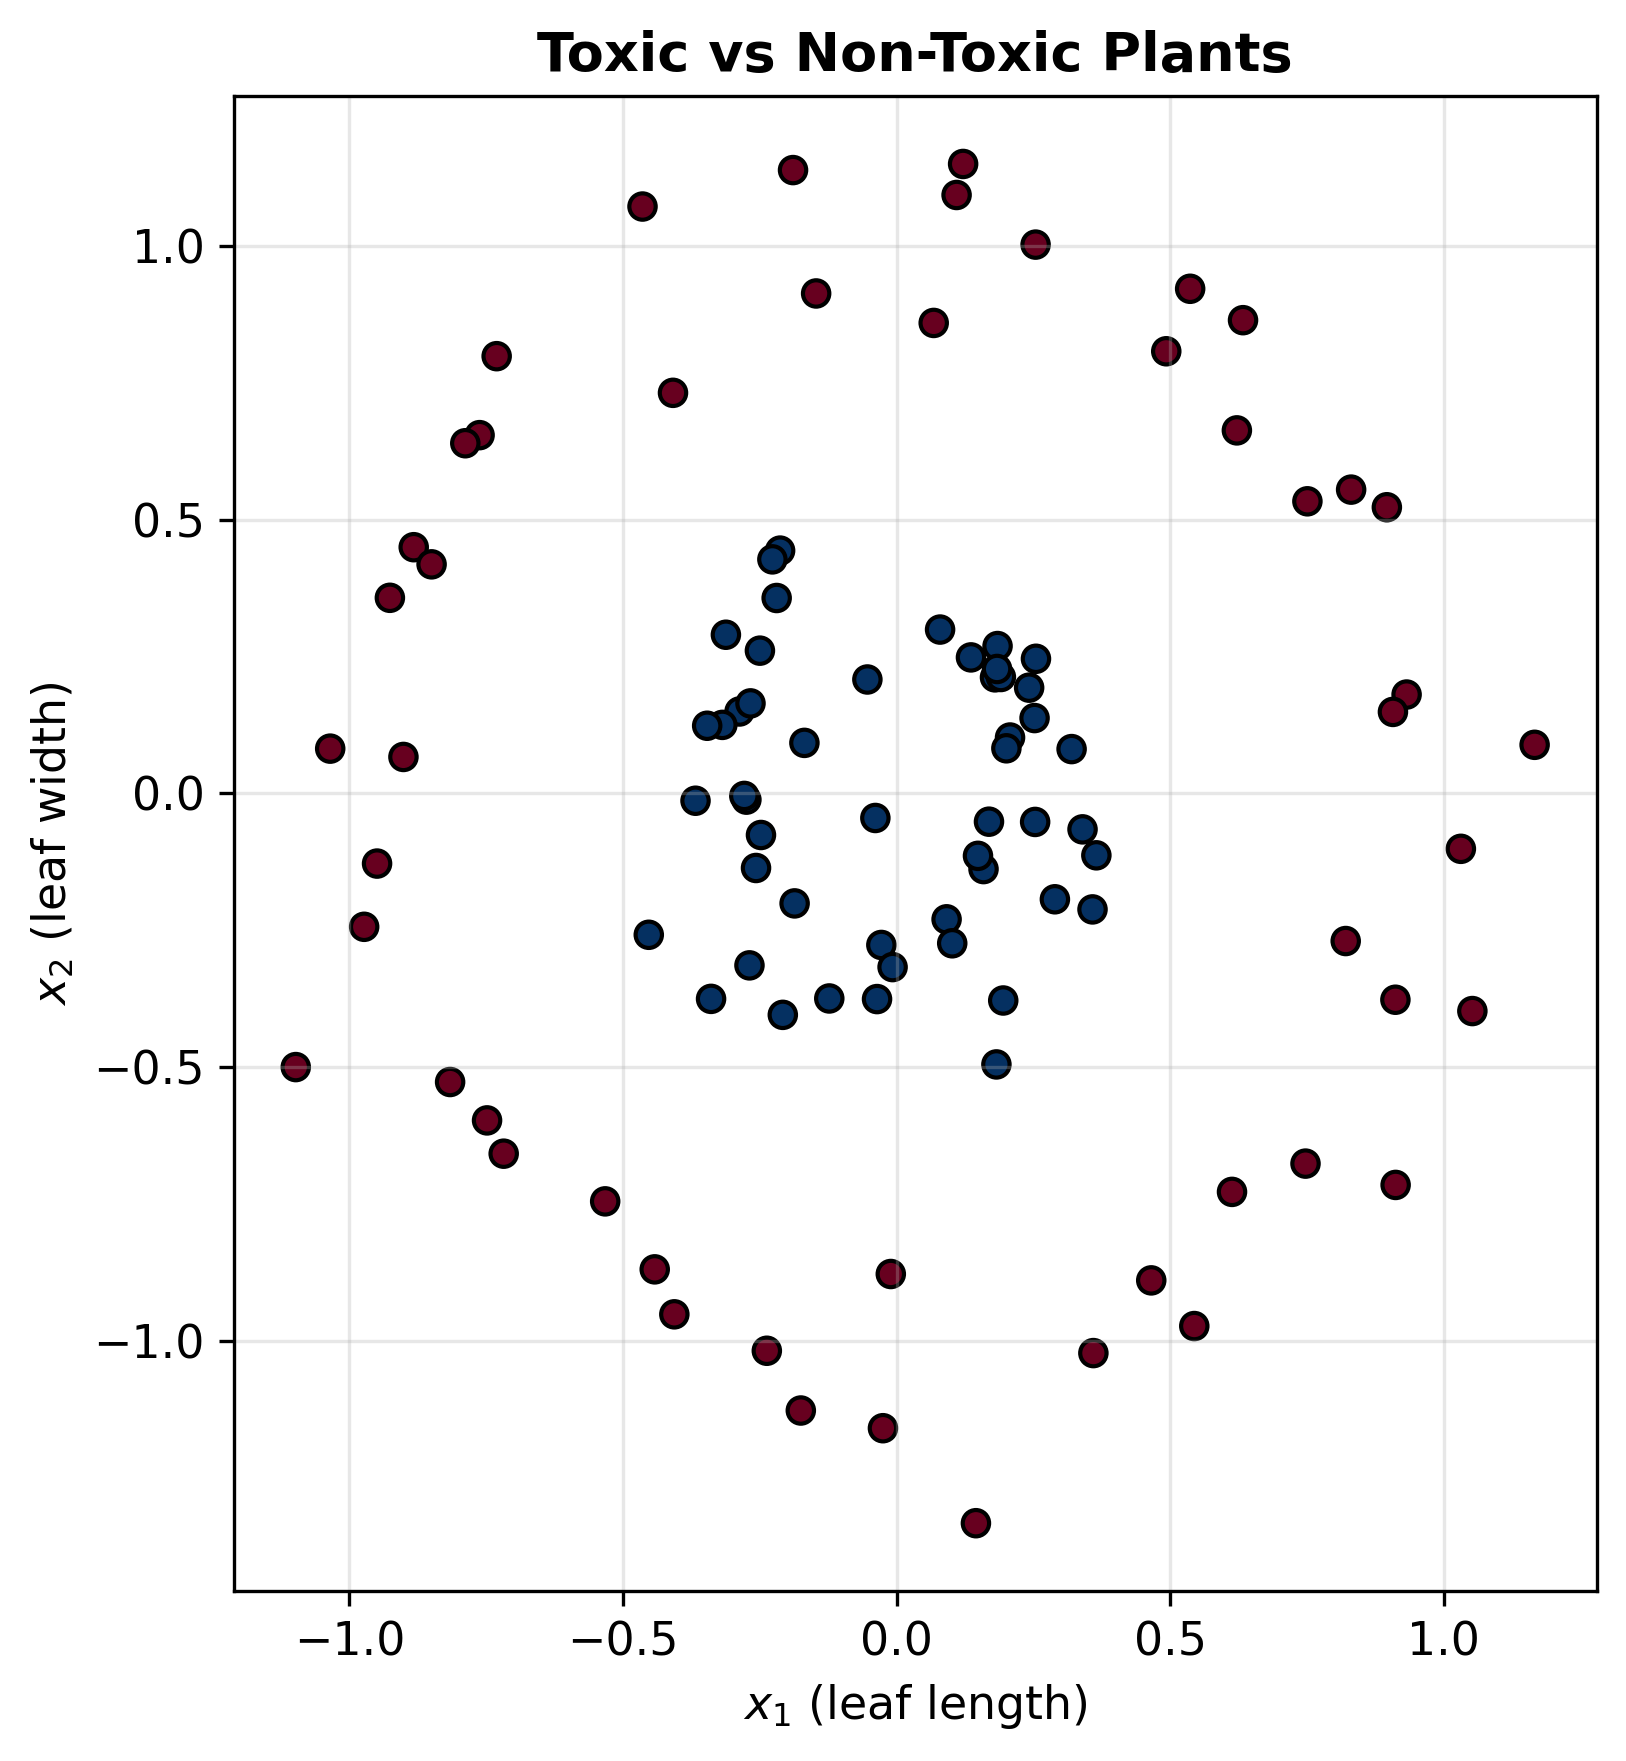
\includegraphics[width=0.55\textwidth]{images/dataset.png}
    \caption{Two classes of data arranged in concentric circles --- impossible to separate with a straight line. Generated from \texttt{make\_circles} with \texttt{n\_samples=100}, \texttt{noise=0.1}, \texttt{factor=0.3}.}
\end{figure}

The two colors represent the two classes: one forms an inner cluster, the other a ring around it.

No straight line can separate them. A single neuron would fail here.

\begin{insightbox}[title=Why This Matters]
This is exactly the kind of problem that requires a \textbf{neural network}.
A single neuron draws a line. A network draws curves.

The data comes from \texttt{sklearn.datasets.make\_circles} --- a classic toy dataset for testing nonlinear classifiers.
\end{insightbox}

In code, we generate it like this:

\begin{lstlisting}
from sklearn.datasets import make_circles

X, y = make_circles(n_samples=100, noise=0.1, factor=0.3, random_state=0)
X = X.T                           # shape: (2, 100)
y = y.reshape((1, y.shape[0]))    # shape: (1, 100)
\end{lstlisting}

\begin{defbox}[title=Convention: Data Shape]
Throughout this episode, we follow this convention:
\begin{itemize}
  \item $X$ has shape \texttt{(n\_features, n\_samples)} --- each column is one data point
  \item $y$ has shape \texttt{(1, n\_samples)} --- one label per sample
\end{itemize}
This is the standard layout for vectorized neural network computation.
\end{defbox}

%% ============================================================
%% SECTION 3 — INITIALIZATION
%% ============================================================
\section{Initialization --- Giving the Network a Body}

Before the network can learn anything, it needs a \textbf{structure}.

We need to decide:
\begin{enumerate}
  \item \textbf{How many inputs?} That's determined by the data --- here, $n_0 = 2$.
  \item \textbf{How many hidden neurons?} We choose this --- let's start with $n_1 = 32$.
  \item \textbf{How many outputs?} Binary classification means $n_2 = 1$.
\end{enumerate}

\begin{figure}[H]
    \centering
    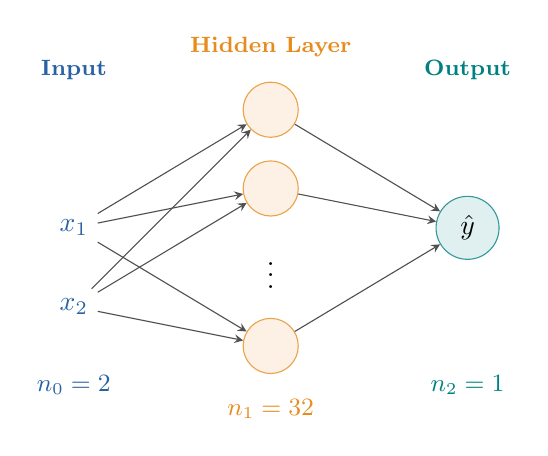
\begin{tikzpicture}[x=2.5cm, y=1cm, >=stealth]

    % Input layer
    \node[font=\bfseries, text=inputblue] at (0, 1.5) (x1) {$x_1$};
    \node[font=\bfseries, text=inputblue] at (0, 0.5) (x2) {$x_2$};
    \node[text=inputblue, font=\small] at (0, -0.5) {$n_0 = 2$};

    % Hidden layer (simplified)
    \node[circle, draw=neuronorange!80, fill=neuronorange!12, minimum size=0.7cm] at (1, 3) (h1) {};
    \node[circle, draw=neuronorange!80, fill=neuronorange!12, minimum size=0.7cm] at (1, 2) (h2) {};
    \node at (1, 1) {$\vdots$};
    \node[circle, draw=neuronorange!80, fill=neuronorange!12, minimum size=0.7cm] at (1, 0) (hn) {};
    \node[text=neuronorange, font=\small] at (1, -0.8) {$n_1 = 32$};

    % Output layer
    \node[circle, draw=outputlayercolor!80, fill=outputlayercolor!12, minimum size=0.8cm] at (2, 1.5) (out) {$\hat{y}$};
    \node[text=outputlayercolor, font=\small] at (2, -0.5) {$n_2 = 1$};

    % Arrows input -> hidden
    \foreach \h in {h1, h2, hn} {
        \draw[->, arrowgray] (x1) -- (\h);
        \draw[->, arrowgray] (x2) -- (\h);
    }

    % Arrows hidden -> output
    \foreach \h in {h1, h2, hn} {
        \draw[->, arrowgray] (\h) -- (out);
    }

    % Layer labels
    \node[font=\footnotesize, text=inputblue] at (0, 3.5) {\textbf{Input}};
    \node[font=\footnotesize, text=neuronorange] at (1, 3.8) {\textbf{Hidden Layer}};
    \node[font=\footnotesize, text=outputlayercolor] at (2, 3.5) {\textbf{Output}};

    \end{tikzpicture}
    \caption{Architecture of our two-layer neural network: 2 inputs, 32 hidden neurons, 1 output.}
\end{figure}

Now we need to create the \textbf{parameters} for each layer:

\begin{itemize}
  \item \textbf{Layer 1} (input $\to$ hidden): weight matrix $W_1$ of shape $(n_1, n_0)$ and bias $b_1$ of shape $(n_1, 1)$
  \item \textbf{Layer 2} (hidden $\to$ output): weight matrix $W_2$ of shape $(n_2, n_1)$ and bias $b_2$ of shape $(n_2, 1)$
\end{itemize}

\begin{defbox}[title=Why Random Initialization?]
We initialize weights \textbf{randomly} --- not to zero.

If all weights started at zero, every neuron would compute the exact same thing.
They'd all have the same gradients, the same updates, and they'd stay identical forever.

Random initialization \textbf{breaks the symmetry}: each neuron starts differently, learns differently, and becomes useful.
\end{defbox}

Here's the code:

\begin{lstlisting}
def initialization(n0, n1, n2):
    W1 = np.random.randn(n1, n0)   # (32, 2)
    b1 = np.random.randn(n1, 1)    # (32, 1)
    W2 = np.random.randn(n2, n1)   # (1, 32)
    b2 = np.random.randn(n2, 1)    # (1, 1)

    parameters = {
        'W1': W1, 'b1': b1,
        'W2': W2, 'b2': b2
    }
    return parameters
\end{lstlisting}

\begin{insightbox}[title=Checkpoint: Dimensions]
Always check your matrix shapes. This is the number one source of bugs in neural network code.

\begin{center}
\begin{tabular}{l c l}
\textbf{Parameter} & \textbf{Shape} & \textbf{Why} \\
\hline
$W_1$ & $(n_1, n_0)$ & $n_1$ neurons, each with $n_0$ weights \\
$b_1$ & $(n_1, 1)$ & one bias per neuron in layer 1 \\
$W_2$ & $(n_2, n_1)$ & $n_2$ outputs, each connected to $n_1$ neurons \\
$b_2$ & $(n_2, 1)$ & one bias per output neuron \\
\end{tabular}
\end{center}
\end{insightbox}

That's it. Four matrices. The network now has a body.

It doesn't know anything yet --- but it \textit{exists}.

%% ============================================================
%% SECTION 4 — FORWARD PROPAGATION
%% ============================================================
\section{Forward Propagation --- The First Breath}

Now we send data through the network for the first time.

This is \textbf{forward propagation}: the process of computing the output of each layer from input to output, one layer at a time.

\begin{recapbox}[title=From Episode V]
Forward propagation for a two-layer network:

\textit{Note: Episode V used \texttt{tanh} in the hidden layer. In this episode, we use sigmoid in both layers for implementation simplicity; the forward/backprop structure stays the same.}

\textbf{Layer 1:}
\[
Z_1 = W_1 \cdot X + b_1 \qquad A_1 = \sigma(Z_1)
\]

\textbf{Layer 2 (output):}
\[
Z_2 = W_2 \cdot A_1 + b_2 \qquad A_2 = \sigma(Z_2)
\]

$A_2$ is the network's prediction.
\end{recapbox}

In Python, this becomes:

\begin{lstlisting}
def forward_propagation(X, parameters):
    W1 = parameters['W1']
    b1 = parameters['b1']
    W2 = parameters['W2']
    b2 = parameters['b2']

    # Layer 1
    Z1 = W1.dot(X) + b1            # Linear transformation
    A1 = 1 / (1 + np.exp(-Z1))     # Sigmoid activation

    # Layer 2 (output)
    Z2 = W2.dot(A1) + b2           # Linear transformation
    A2 = 1 / (1 + np.exp(-Z2))     # Sigmoid activation

    activations = {'A1': A1, 'A2': A2}
    return activations
\end{lstlisting}

\textbf{That's it.}

Six lines of actual computation. Same architecture as Episode V --- now alive.

\begin{insightbox}[title=Tracing the Dimensions]
Let's follow the shapes through the network step by step:
\begin{center}
\begin{tabular}{l c l}
\textbf{Operation} & \textbf{Shape} & \textbf{Explanation} \\
\hline
$X$ & $(2, 100)$ & 2 features, 100 samples \\
$W_1 \cdot X$ & $(32, 2) \times (2, 100) = (32, 100)$ & \\
$Z_1$ & $(32, 100)$ & 32 neurons, 100 samples \\
$A_1 = \sigma(Z_1)$ & $(32, 100)$ & activations of hidden layer \\
$W_2 \cdot A_1$ & $(1, 32) \times (32, 100) = (1, 100)$ & \\
$A_2 = \sigma(Z_2)$ & $(1, 100)$ & one prediction per sample \\
\end{tabular}
\end{center}

If any shape doesn't match, NumPy will tell you immediately.
\end{insightbox}

The network just took its first breath.

It processed 100 data points through 32 neurons, passed through two layers of activation,
and produced 100 predictions --- all in a fraction of a second.

The predictions are garbage right now (random weights, remember?).

But that's about to change.

%% ============================================================
%% SECTION 5 — BACKPROPAGATION
%% ============================================================
\section{Backpropagation --- Learning from Mistakes}

This is the moment where everything comes together.

In Episode V, you derived the gradients of the loss with respect to every parameter.
You spent pages computing $\frac{\partial \mathcal{L}}{\partial W_2}$, $\frac{\partial \mathcal{L}}{\partial b_2}$,
$\frac{\partial \mathcal{L}}{\partial W_1}$, $\frac{\partial \mathcal{L}}{\partial b_1}$.

Let's see what all that math looks like in code.

\subsection{The Cost Function}

First, we need to measure how wrong the network is.

We use the same \textbf{log-loss} (binary cross-entropy) as always:

\[
\mathcal{L} = -\frac{1}{m} \sum_{i=1}^{m} \left[ y^{(i)} \log(A_2^{(i)}) + (1 - y^{(i)}) \log(1 - A_2^{(i)}) \right]
\]

In code:

\begin{lstlisting}
def log_loss(A, y):
    m = y.shape[1]
    epsilon = 1e-15   # prevent log(0)
    return -1/m * np.sum(
        y * np.log(A + epsilon) +
        (1 - y) * np.log(1 - A + epsilon)
    )
\end{lstlisting}

\subsection{The Gradient Equations}

Now, the gradients. Here they are --- side by side with their code.
Episode V used \texttt{tanh} in the hidden layer, while here we use sigmoid:
the backprop pattern is identical, only the hidden activation derivative changes.

\begin{resultbox}[title=Episode V Equations $\to$ Python Code]

\textbf{Output layer gradients:}
\[
dZ_2 = A_2 - y \qquad dW_2 = \frac{1}{m} \, dZ_2 \cdot A_1^\top \qquad db_2 = \frac{1}{m} \sum dZ_2
\]

\textbf{Hidden layer gradients:}
\[
dZ_1 = W_2^\top \cdot dZ_2 \circ A_1 \circ (1 - A_1) \qquad dW_1 = \frac{1}{m} \, dZ_1 \cdot X^\top \qquad db_1 = \frac{1}{m} \sum dZ_1
\]
\end{resultbox}

And the code:

\begin{lstlisting}
def back_propagation(X, y, parameters, activations):
    A1 = activations['A1']
    A2 = activations['A2']
    W2 = parameters['W2']
    m = y.shape[1]

    # Output layer
    dZ2 = A2 - y
    dW2 = 1/m * dZ2.dot(A1.T)
    db2 = 1/m * np.sum(dZ2, axis=1, keepdims=True)

    # Hidden layer
    dZ1 = np.dot(W2.T, dZ2) * A1 * (1 - A1)
    dW1 = 1/m * dZ1.dot(X.T)
    db1 = 1/m * np.sum(dZ1, axis=1, keepdims=True)

    gradients = {
        'dW1': dW1, 'db1': db1,
        'dW2': dW2, 'db2': db2
    }
    return gradients
\end{lstlisting}

Count the lines.

Six lines of gradient computation. That's it.

\textit{This is why you did the math.}

\begin{warnbox}[title=The Hadamard Product]
Notice the \texttt{*} operator in the $dZ_1$ line. This is the element-wise product (Hadamard product), denoted $\circ$ in math.

It's \textbf{not} a matrix multiplication --- it's component-by-component.

\texttt{np.dot()} is matrix multiplication. \texttt{*} is element-wise.

Getting this wrong is a classic bug.
\end{warnbox}

Let's take a moment to appreciate what just happened.

In Episode V, we spent several pages deriving $dZ_1$ through the chain rule.
We went from $\frac{\partial \mathcal{L}}{\partial A_2}$ to $\frac{\partial \mathcal{L}}{\partial Z_2}$ to $\frac{\partial \mathcal{L}}{\partial A_1}$ to $\frac{\partial \mathcal{L}}{\partial Z_1}$.

All of that --- \textbf{one line of code}:

\begin{lstlisting}
dZ1 = np.dot(W2.T, dZ2) * A1 * (1 - A1)
\end{lstlisting}

\begin{insightbox}[title=Theory $\to$ Code]
This is the pattern of deep learning engineering:
\begin{enumerate}
  \item Derive the math \textbf{once} (Episode V)
  \item Translate it into code \textbf{once} (this episode)
  \item Never touch it again --- frameworks will do it for you
\end{enumerate}

But you need to understand it. \textbf{That's what makes you dangerous.}
\end{insightbox}

%% ============================================================
%% SECTION 6 — UPDATE & PREDICTION
%% ============================================================
\section{Update and Prediction --- Closing the Loop}

Two more functions and we're done building.

\subsection{Update --- Four Subtractions}

Now that we have the gradients, we update the parameters.

This is \textbf{gradient descent}: move each parameter in the direction that reduces the loss.

\[
W \leftarrow W - \alpha \cdot dW \qquad b \leftarrow b - \alpha \cdot db
\]

where $\alpha$ is the \textbf{learning rate} --- how big each step is.

\begin{lstlisting}
def update(gradients, parameters, learning_rate):
    W1 = parameters['W1'] - learning_rate * gradients['dW1']
    b1 = parameters['b1'] - learning_rate * gradients['db1']
    W2 = parameters['W2'] - learning_rate * gradients['dW2']
    b2 = parameters['b2'] - learning_rate * gradients['db2']

    parameters = {
        'W1': W1, 'b1': b1,
        'W2': W2, 'b2': b2
    }
    return parameters
\end{lstlisting}

Four subtractions. That's learning.

\begin{warnbox}[title=The Learning Rate]
Too high and the network overshoots, oscillating wildly around the minimum.
Too low and it barely moves, taking forever to converge.

There's no formula to pick the right $\alpha$. You try, you observe, you adjust.

That's part of the craft.
\end{warnbox}

\subsection{Prediction --- Making Decisions}

The network outputs a continuous value $A_2 \in [0, 1]$ --- a probability.

To turn it into a decision, we apply a \textbf{threshold}:

\[
\hat{y} = \begin{cases} 1 & \text{if } A_2 \geq 0.5 \\ 0 & \text{otherwise} \end{cases}
\]

\begin{lstlisting}
def predict(X, parameters):
    activations = forward_propagation(X, parameters)
    A2 = activations['A2']
    return A2 >= 0.5
\end{lstlisting}

We compute accuracy by comparing predictions to true labels:

\begin{lstlisting}
from sklearn.metrics import accuracy_score

y_pred = predict(X, parameters)
accuracy = accuracy_score(y.flatten(), y_pred.flatten())
\end{lstlisting}

\begin{insightbox}[title=Why 0.5?]
At $A_2 = 0.5$, the network is maximally uncertain --- it has no preference between class 0 and class 1.
Above 0.5, it leans toward class 1. Below, class 0.

This threshold is a design choice. In some applications (e.g., medical diagnosis), you might lower it to catch more positives --- even at the cost of more false alarms.
\end{insightbox}

%% ============================================================
%% CHECKPOINT
%% ============================================================
\begin{recapbox}[title=Checkpoint --- Your Toolkit So Far]
Before going further, let's take stock.
You have written \textbf{seven functions} from scratch, each handling one piece of the puzzle:

\begin{center}
\renewcommand{\arraystretch}{1.3}
\begin{tabular}{r l l}
\textbf{\#} & \textbf{Function} & \textbf{Role} \\
\hline
1 & \texttt{initialization} & Create $W$ and $b$ with random values \\
2 & \texttt{forward\_propagation} & $X \to Z_1 \to A_1 \to Z_2 \to A_2$ \\
3 & \texttt{log\_loss} & Measure how wrong the network is \\
4 & \texttt{back\_propagation} & Compute all gradients \\
5 & \texttt{update} & Adjust parameters via gradient descent \\
6 & \texttt{predict} & Turn probabilities into decisions \\
7 & \texttt{neural\_network} & Orchestrate everything (next section) \\
\end{tabular}
\end{center}

Nothing here was imported from a library. Every line is yours.
\end{recapbox}

%% ============================================================
%% SECTION 7 — TRAINING LOOP
%% ============================================================
\section{The Training Loop --- Putting It All Together}

We have all the pieces. Let's assemble them.

The training loop repeats the same four steps over and over:

\begin{enumerate}
  \item \textbf{Forward propagation} --- compute predictions
  \item \textbf{Cost} --- measure the error
  \item \textbf{Backpropagation} --- compute gradients
  \item \textbf{Update} --- adjust parameters
\end{enumerate}

Each iteration is called an \textbf{epoch}.

\begin{figure}[H]
    \centering
    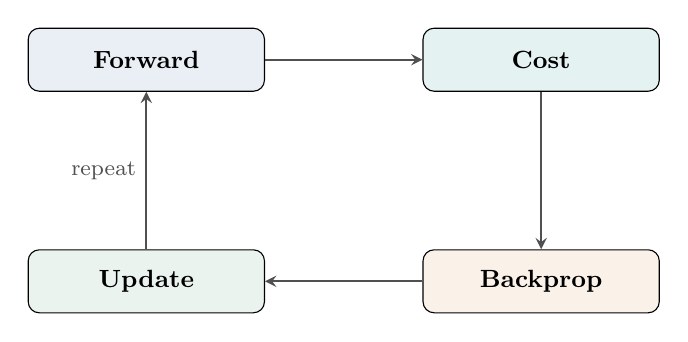
\begin{tikzpicture}[node distance=2cm, >=stealth, every node/.style={font=\small}]
        \node[draw, rounded corners, fill=defblue!10, minimum width=3cm, minimum height=0.8cm] (fw) {\textbf{Forward}};
        \node[draw, rounded corners, fill=resultteal!10, minimum width=3cm, minimum height=0.8cm, right=of fw] (cost) {\textbf{Cost}};
        \node[draw, rounded corners, fill=warnorange!10, minimum width=3cm, minimum height=0.8cm, below=of cost] (bp) {\textbf{Backprop}};
        \node[draw, rounded corners, fill=activgreen!10, minimum width=3cm, minimum height=0.8cm, left=of bp] (up) {\textbf{Update}};

        \draw[->, thick, arrowgray] (fw) -- (cost);
        \draw[->, thick, arrowgray] (cost) -- (bp);
        \draw[->, thick, arrowgray] (bp) -- (up);
        \draw[->, thick, arrowgray] (up) -- (fw) node[midway, left] {\footnotesize repeat};
    \end{tikzpicture}
    \caption{The training loop: four steps, repeated for each epoch.}
\end{figure}

\begin{lstlisting}
def neural_network(X, y, n1=32, learning_rate=0.1, n_epochs=1000):
    # Dimensions
    n0 = X.shape[0]
    n2 = y.shape[0]

    # Initialize
    np.random.seed(0)
    parameters = initialization(n0, n1, n2)

    # Training history
    train_loss = []
    train_acc = []

    for i in range(n_epochs):
        # 1. Forward
        activations = forward_propagation(X, parameters)
        A2 = activations['A2']

        # 2. Cost
        loss = log_loss(A2, y)
        train_loss.append(loss)

        # 3. Accuracy
        y_pred = predict(X, parameters)
        acc = accuracy_score(y.flatten(), y_pred.flatten())
        train_acc.append(acc)

        # 4. Backprop
        gradients = back_propagation(X, y, parameters, activations)

        # 5. Update
        parameters = update(gradients, parameters, learning_rate)

    return parameters, train_loss, train_acc
\end{lstlisting}

Let's train:

\begin{lstlisting}
parameters, train_loss, train_acc = neural_network(
    X, y, n1=32, learning_rate=0.1, n_epochs=1000
)
\end{lstlisting}

\begin{insightbox}[title=What Happens Inside]
At each epoch:
\begin{itemize}
  \item The loss should \textbf{decrease} --- the network is making smaller errors
  \item The accuracy should \textbf{increase} --- the network is classifying more correctly
  \item The weights are being nudged, slowly, toward the right values
\end{itemize}

If the loss increases or oscillates wildly, the learning rate is probably too high.
\end{insightbox}

After 1000 epochs with 32 hidden neurons and a learning rate of 0.1:

\begin{figure}[H]
    \centering
    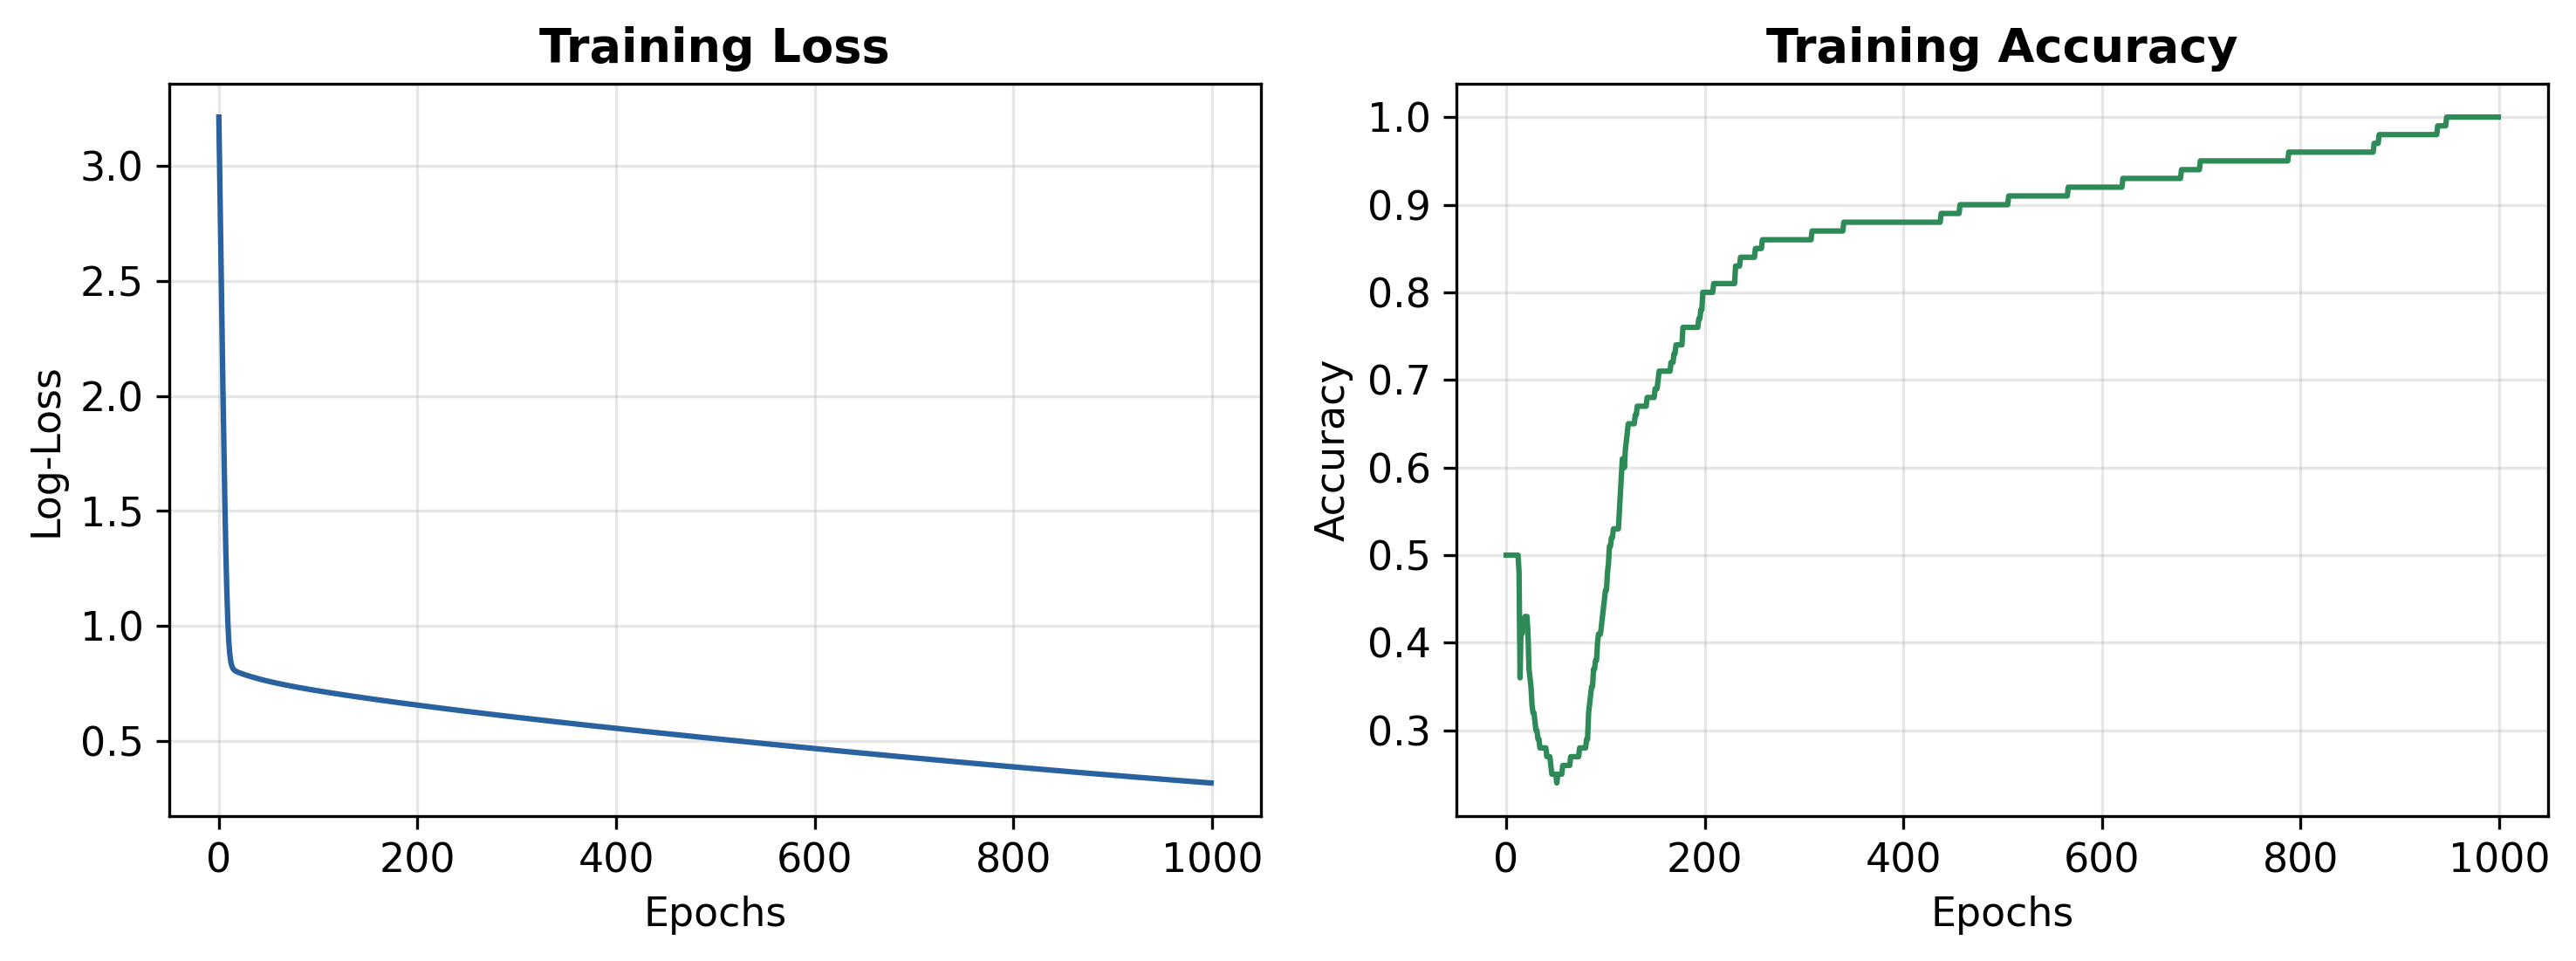
\includegraphics[width=0.92\textwidth]{images/training_curves.png}
    \caption{Training on \texttt{make\_circles}: the loss drops sharply while accuracy climbs toward 100\%.}
\end{figure}

\textbf{The network learned.}

From random weights to near-perfect classification --- in a few seconds.

%% ============================================================
%% SECTION 9 — DECISION BOUNDARY
%% ============================================================
\section{Decision Boundary --- Seeing Intelligence}

Let's visualize \textit{what} the network learned.

The \textbf{decision boundary} is the set of points where the network is equally uncertain:
$A_2 = 0.5$, meaning $Z_2 = 0$, meaning $W_2 \cdot A_1 + b_2 = 0$.

For a single neuron, this boundary is a straight line.

For a network? It's a \textbf{curve}.

\begin{figure}[H]
\centering
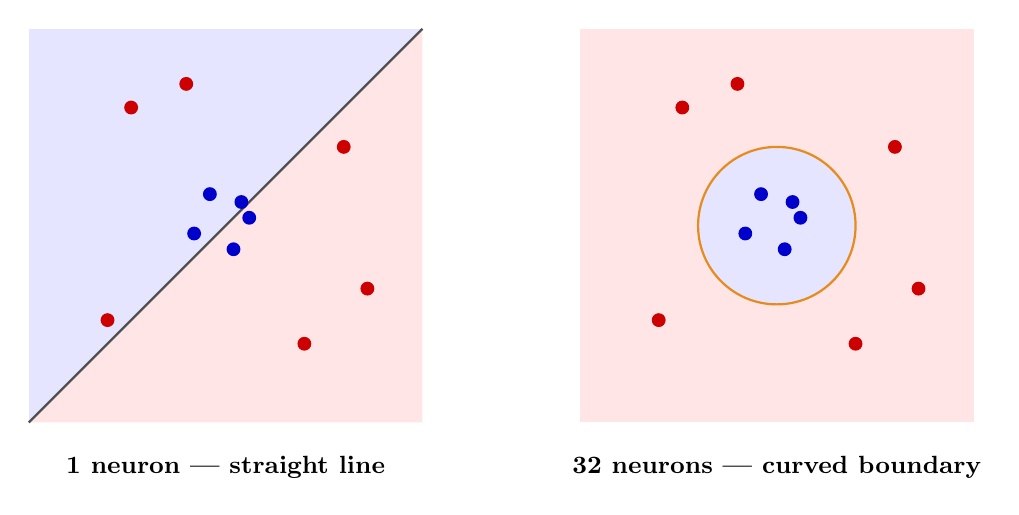
\begin{tikzpicture}
  % --- Left: single neuron (linear) ---
  \begin{scope}
    \fill[blue!10] (-2.5,-2.5) rectangle (2.5,2.5);
    \fill[red!10] (-2.5,-2.5) -- (2.5,-2.5) -- (2.5,2.5) -- (-2.5,-2.5);
    \draw[arrowgray, thick] (-2.5,-2.5) -- (2.5,2.5);
    % data points class 0 (inner ring - misclassified in linear)
    \foreach \x/\y in {0.3/0.1, -0.2/0.4, 0.1/-0.3, -0.4/-0.1, 0.2/0.3}{
      \fill[blue!80!black] (\x,\y) circle (2.5pt);
    }
    % data points class 1 (outer ring)
    \foreach \x/\y in {1.5/1.0, -1.2/1.5, 1.8/-0.8, -1.5/-1.2, -0.5/1.8, 1.0/-1.5}{
      \fill[red!80!black] (\x,\y) circle (2.5pt);
    }
    \node[below, font=\small\bfseries] at (0,-2.8) {1 neuron --- straight line};
  \end{scope}

  % --- Right: network (nonlinear) ---
  \begin{scope}[xshift=7cm]
    \fill[red!10] (-2.5,-2.5) rectangle (2.5,2.5);
    \fill[blue!10] (0,0) circle (1.0);
    \draw[neuronorange, thick] (0,0) circle (1.0);
    % data points class 0 (inner ring - correct)
    \foreach \x/\y in {0.3/0.1, -0.2/0.4, 0.1/-0.3, -0.4/-0.1, 0.2/0.3}{
      \fill[blue!80!black] (\x,\y) circle (2.5pt);
    }
    % data points class 1 (outer ring)
    \foreach \x/\y in {1.5/1.0, -1.2/1.5, 1.8/-0.8, -1.5/-1.2, -0.5/1.8, 1.0/-1.5}{
      \fill[red!80!black] (\x,\y) circle (2.5pt);
    }
    \node[below, font=\small\bfseries] at (0,-2.8) {32 neurons --- curved boundary};
  \end{scope}
\end{tikzpicture}
\caption{Left: a single neuron can only draw a straight line.
Right: a hidden layer with many neurons can learn curved, nonlinear boundaries that wrap around the data.}
\end{figure}

\begin{defbox}[title=How to Plot the Decision Boundary]
\begin{enumerate}
  \item Create a fine grid of points covering the input space
  \item Run every grid point through the trained network
  \item Color each point based on the network's prediction
  \item The boundary appears where the color changes
\end{enumerate}
\end{defbox}

\begin{lstlisting}
def plot_decision_boundary(X, y, parameters):
    x_min, x_max = X[0].min() - 1, X[0].max() + 1
    y_min, y_max = X[1].min() - 1, X[1].max() + 1
    xx, yy = np.meshgrid(
        np.arange(x_min, x_max, 0.01),
        np.arange(y_min, y_max, 0.01)
    )
    grid = np.c_[xx.ravel(), yy.ravel()].T
    Z = predict(grid, parameters)
    Z = Z.reshape(xx.shape)

    plt.contourf(xx, yy, Z, alpha=0.3, cmap='RdBu')
    plt.scatter(X[0], X[1], c=y, cmap='RdBu', edgecolors='k')
    plt.title('Decision Boundary')
    plt.show()
\end{lstlisting}

Run this on our trained model:

\begin{figure}[H]
    \centering
    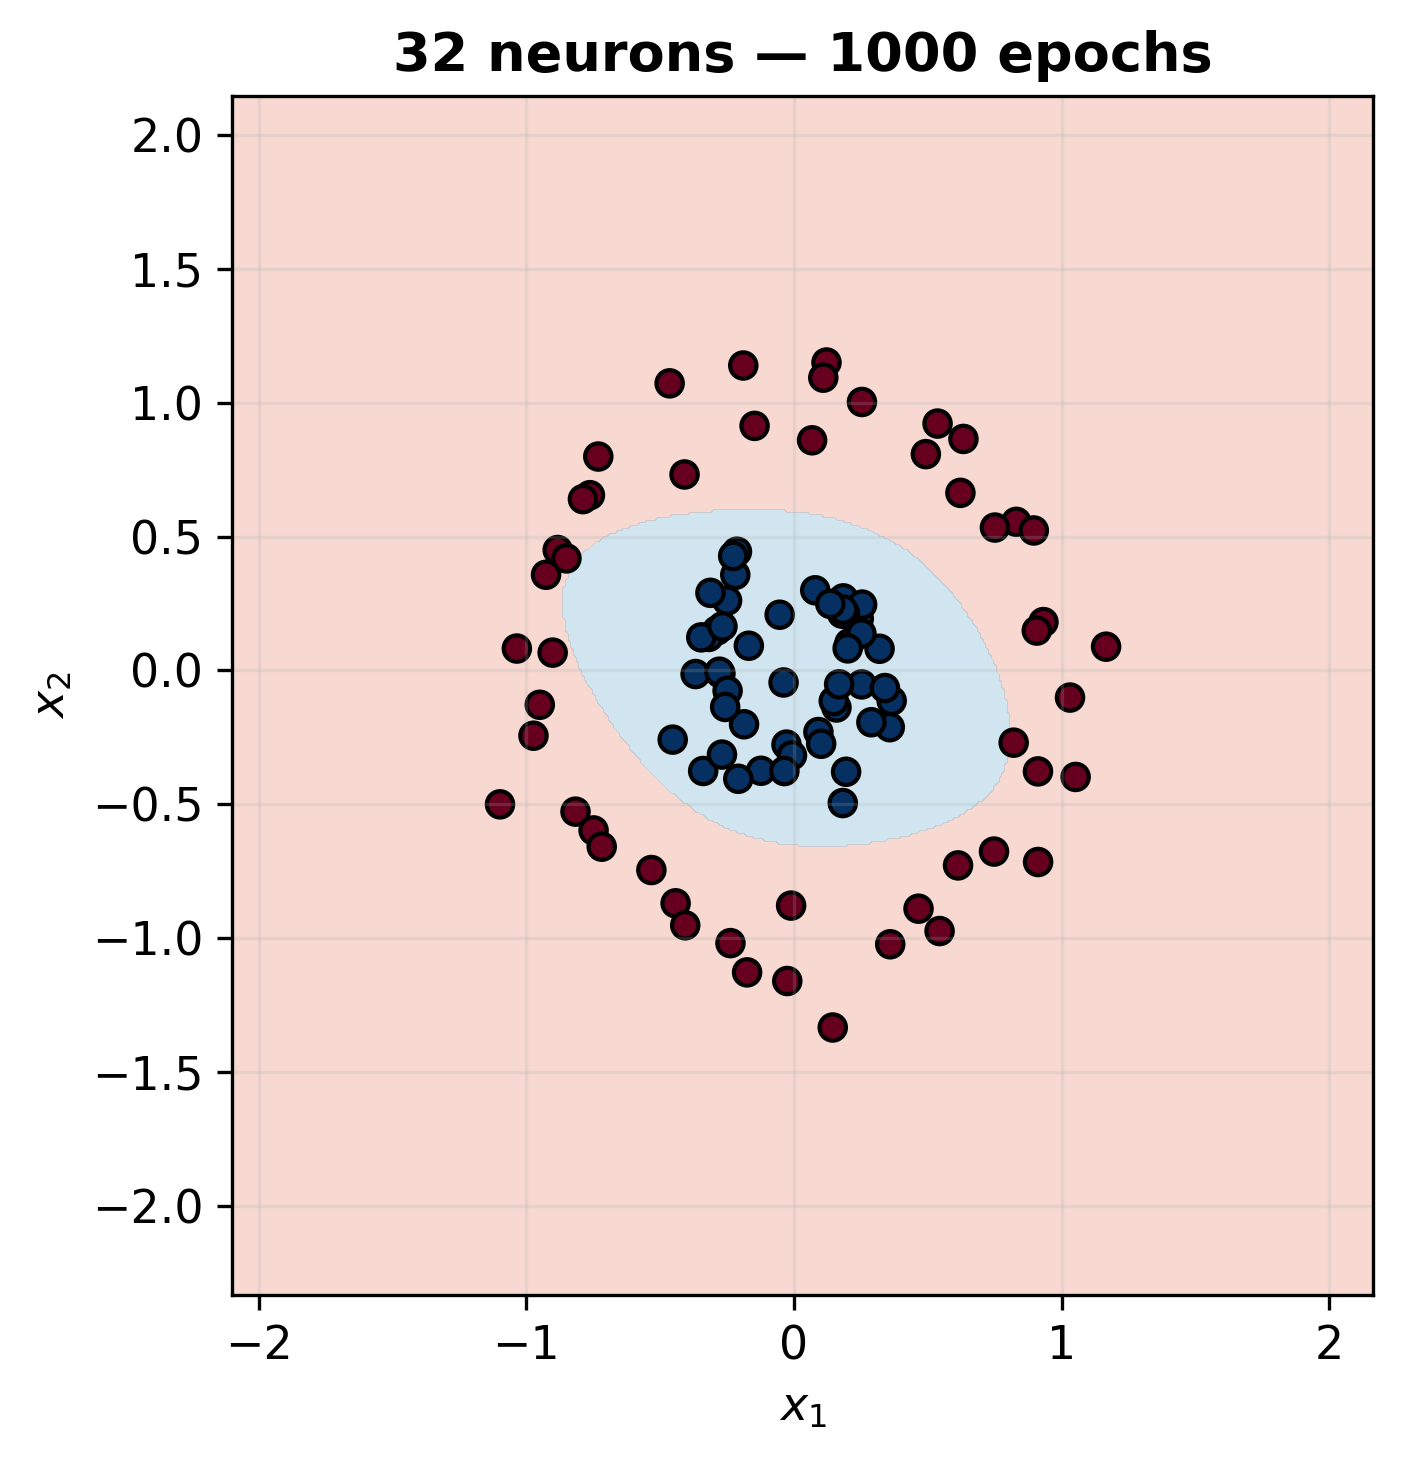
\includegraphics[width=0.48\textwidth]{images/decision_boundary.png}
    \caption{The trained network's decision boundary: a \textbf{nonlinear curve} that wraps around the inner cluster, separating toxic from non-toxic plants with near-perfect precision.}
\end{figure}

\subsection{The Effect of Neuron Count}

What happens when we change $n_1$?

\begin{center}
\begin{tabular}{c l}
\textbf{Neurons} & \textbf{Behavior} \\
\hline
1 & Linear boundary (= logistic regression) \\
2 & Slightly curved, not enough \\
4 & Captures some nonlinearity \\
8 & Clear circular-ish boundary \\
16 & Smooth, accurate separation \\
32 & Near-perfect classification \\
\end{tabular}
\end{center}

\begin{figure}[H]
    \centering
    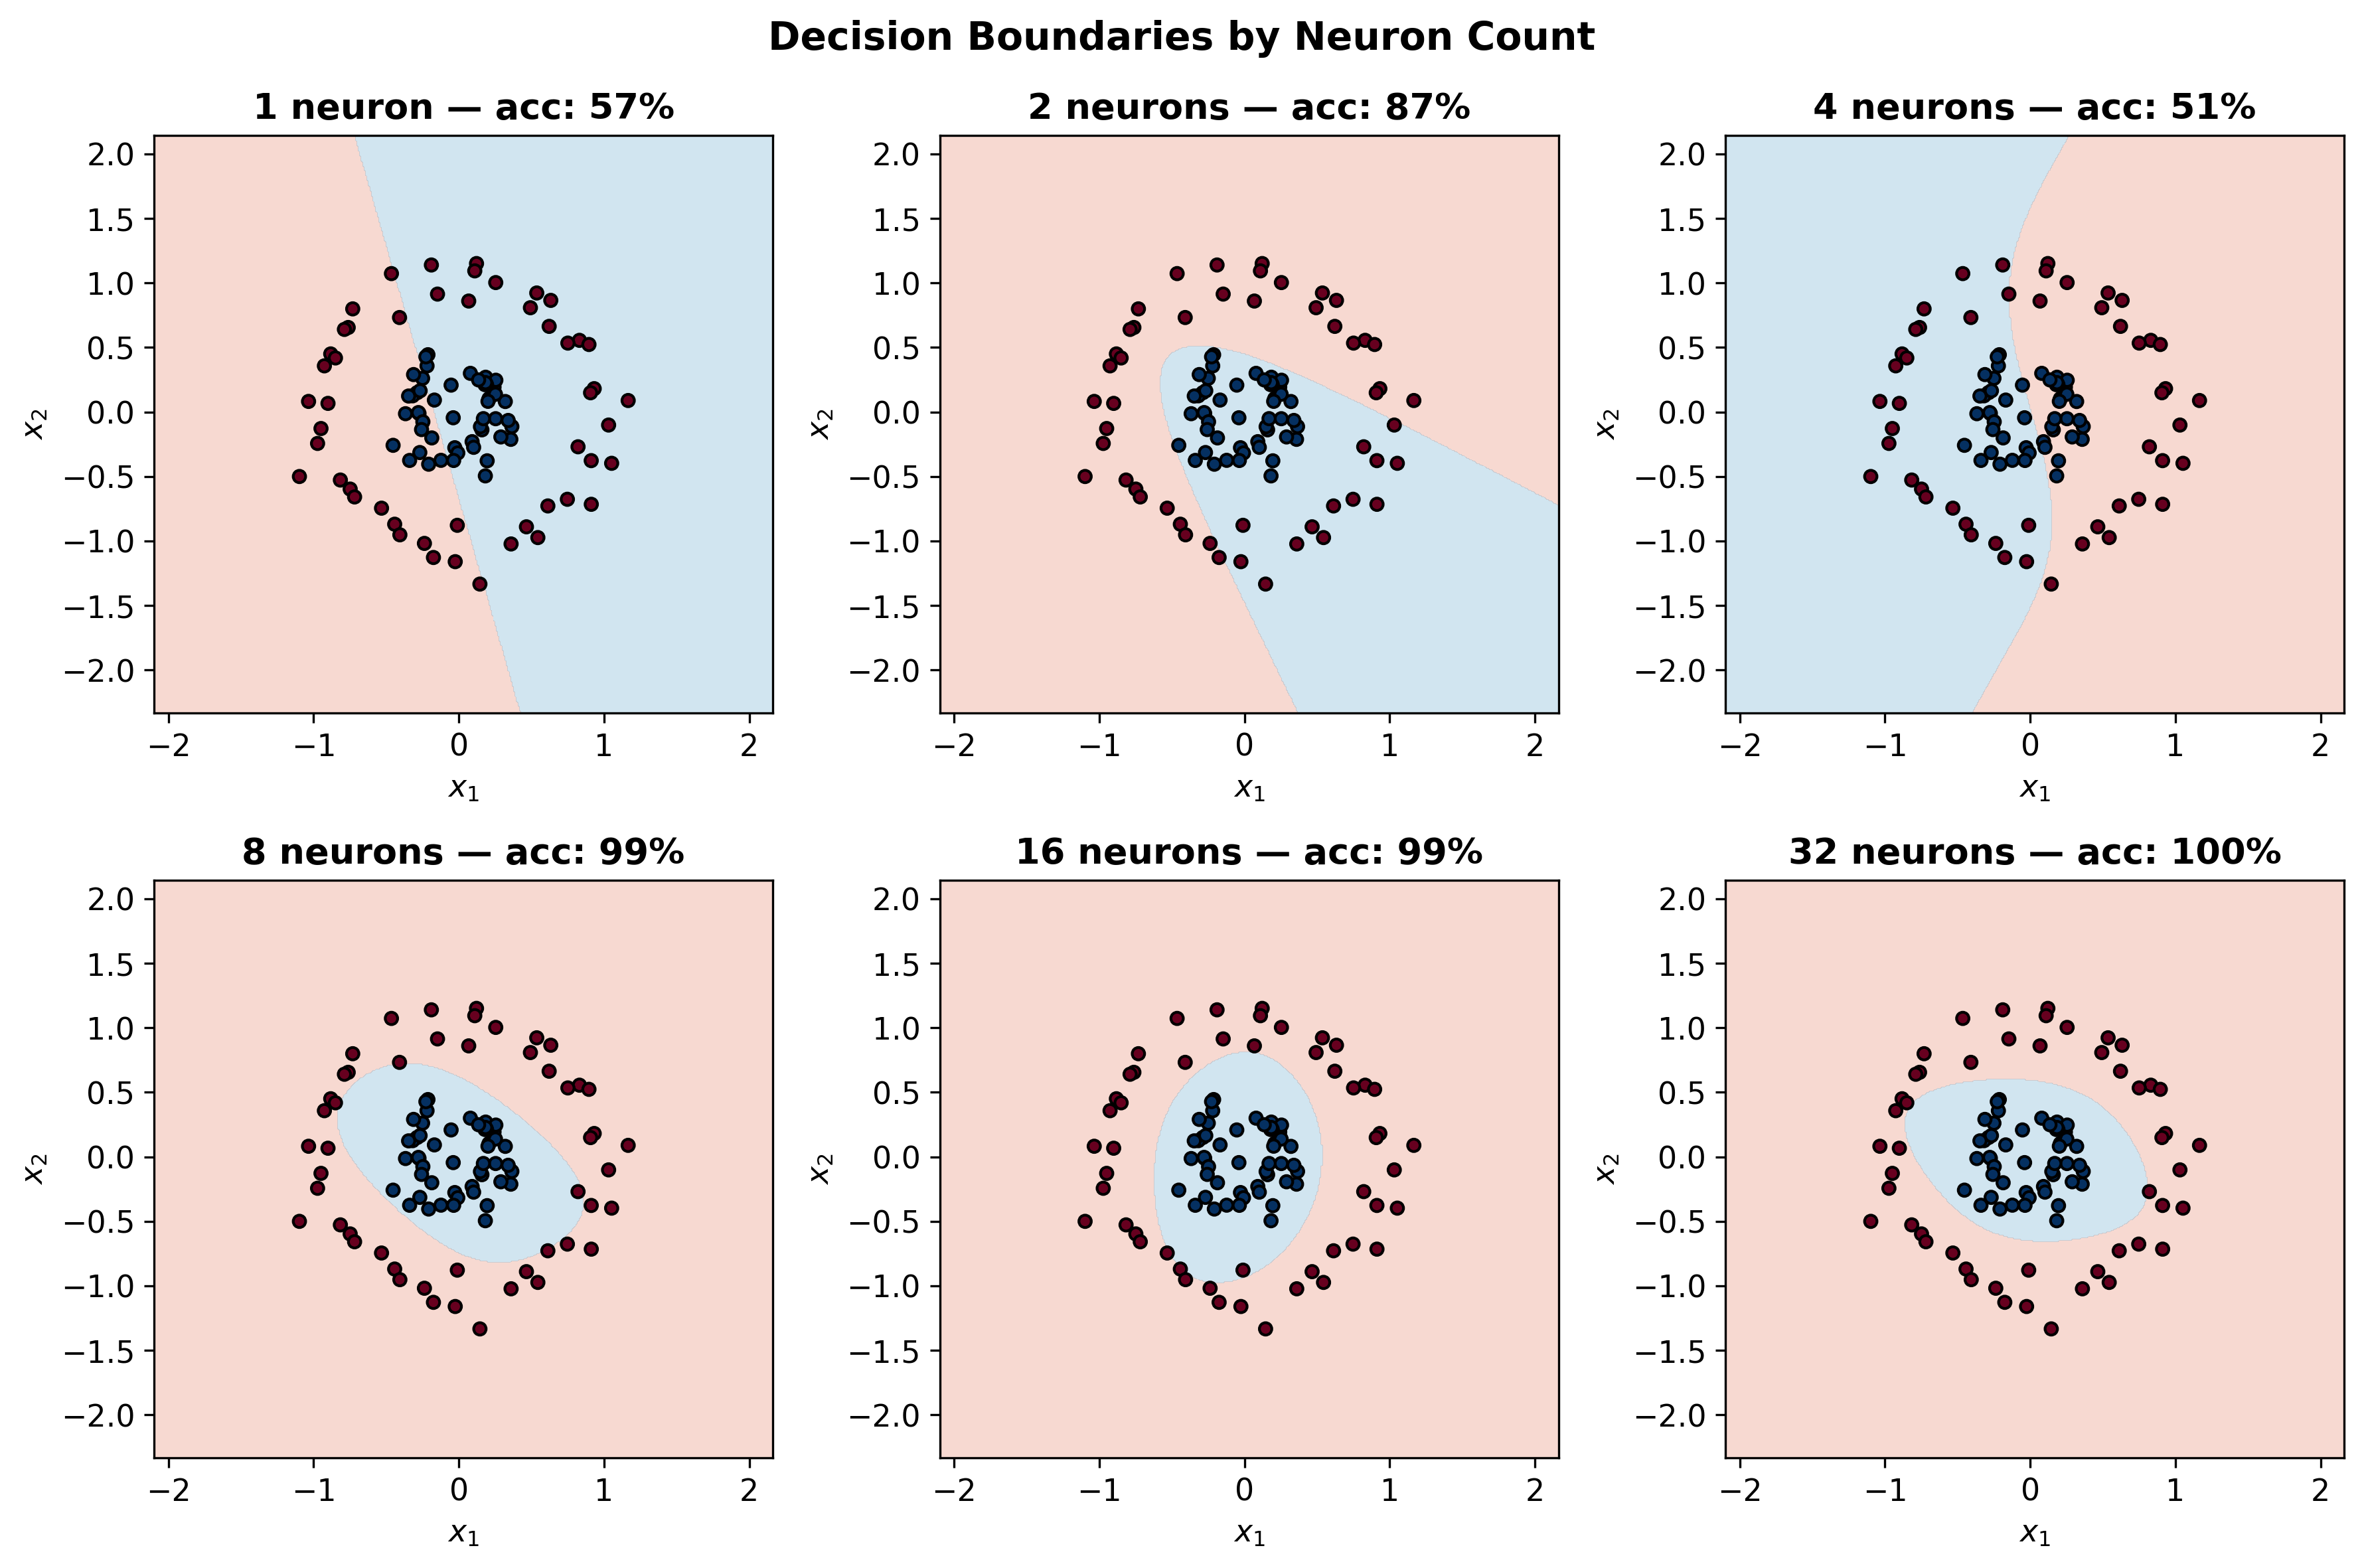
\includegraphics[width=0.95\textwidth]{images/neuron_comparison.png}
    \caption{Decision boundaries for different hidden layer sizes. With 1 neuron, the boundary is a straight line (= logistic regression). As we add neurons, the network carves out increasingly complex, nonlinear boundaries.}
\end{figure}

\begin{insightbox}[title=More Neurons = More Flexibility]
Each neuron in the hidden layer contributes one ``feature'' to the representation.
More neurons means the network can carve out more complex boundaries.

But be careful: too many neurons with too little data leads to \textbf{overfitting} --- a problem we'll encounter very soon.
\end{insightbox}

\textit{This is what intelligence looks like:} the ability to draw the right boundary, automatically, from data alone.

%% ============================================================
%% SECTION 10 — REAL DATA
%% ============================================================
\section{Real Data --- Cats vs Dogs}

Toy datasets are great for learning. But let's see how our network handles real images.

We're going back to the \textbf{cats vs dogs} dataset from Episode IV.

\begin{figure}[H]
    \centering
    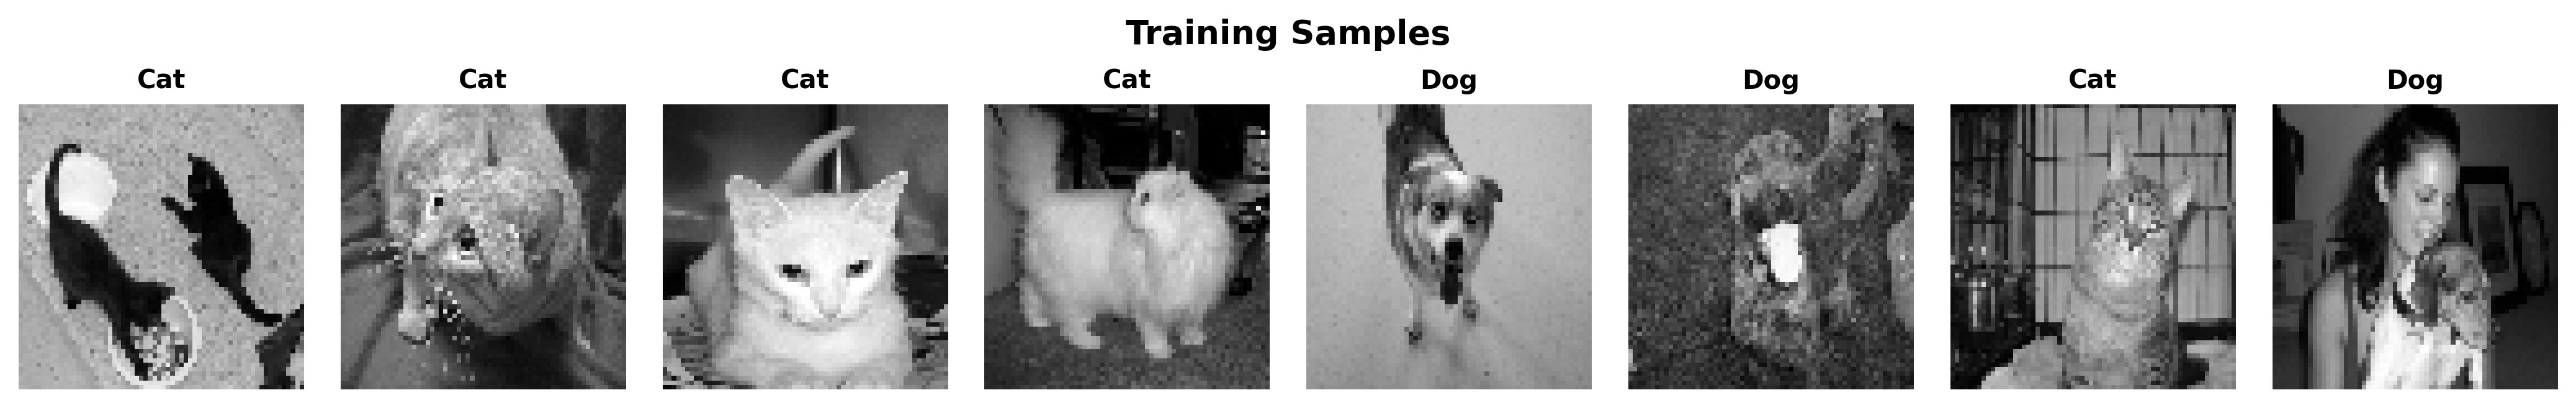
\includegraphics[width=0.85\textwidth]{images/sample_images.png}
    \caption{A few training samples from the cats vs dogs dataset --- 64$\times$64 grayscale images.}
\end{figure}

\subsection{Data Preprocessing}

Before feeding images into a neural network, we need to preprocess them:

\begin{enumerate}
  \item \textbf{Load} the data from HDF5 files
  \item \textbf{Reshape} each 64$\times$64 image into a vector of 4096 pixels
  \item \textbf{Normalize} pixel values to $[0, 1]$ by dividing by 255
  \item \textbf{Transpose} to get shape \texttt{(n\_features, n\_samples)}
\end{enumerate}

\begin{lstlisting}
from src.utilities import load_data

X_train, y_train, X_test, y_test = load_data()

# Reshape: (1000, 64, 64) -> (4096, 1000)
X_train_flat = X_train.reshape(X_train.shape[0], -1).T
X_test_flat = X_test.reshape(X_test.shape[0], -1).T

# Normalize
X_train_flat = X_train_flat / 255.
X_test_flat = X_test_flat / 255.

# Labels: shape (1, n_samples)
y_train = y_train.reshape(1, -1)
y_test = y_test.reshape(1, -1)
\end{lstlisting}

\begin{center}
\begin{tabular}{l c}
\textbf{Data} & \textbf{Shape} \\
\hline
\texttt{X\_train\_flat} & $(4096, 1000)$ \\
\texttt{X\_test\_flat} & $(4096, 200)$ \\
\texttt{y\_train} & $(1, 1000)$ \\
\texttt{y\_test} & $(1, 200)$ \\
\end{tabular}
\end{center}

Each image is now a column vector of 4096 numbers.

\subsection{Training on Images}

Here's the beautiful thing: we use the \textbf{exact same} \texttt{neural\_network} function we wrote for toy circles --- no changes needed.

\begin{lstlisting}
parameters, train_loss, train_acc = neural_network(
    X_train_flat, y_train, n1=64,
    learning_rate=0.1, n_epochs=10000
)
\end{lstlisting}

\begin{insightbox}[title={Same Code, Different World}]
The network doesn't know it's looking at cat photos. It sees
4096 numbers and searches for the pattern that separates class 0 from class 1.

That's the power of abstraction: once the math is right, the data can be anything.
\end{insightbox}

But we want to know more than just training performance.
Does the network \emph{generalize} --- can it classify images it has never seen?

To find out, we modify the training loop to also track test loss and accuracy at each epoch:

\begin{lstlisting}
def neural_network_with_test(X_train, y_train, X_test, y_test,
                             n1=32, learning_rate=0.1, n_epochs=1000):
    n0 = X_train.shape[0]
    n2 = y_train.shape[0]

    np.random.seed(0)
    parameters = initialization(n0, n1, n2)

    train_loss_hist, test_loss_hist = [], []
    train_acc_hist, test_acc_hist = [], []

    for i in range(n_epochs):
        # Forward + cost (train)
        act_train = forward_propagation(X_train, parameters)
        train_loss_hist.append(log_loss(act_train['A2'], y_train))

        # Forward + cost (test)
        act_test = forward_propagation(X_test, parameters)
        test_loss_hist.append(log_loss(act_test['A2'], y_test))

        # Accuracy
        train_acc_hist.append(
            accuracy_score(y_train.flatten(),
                           predict(X_train, parameters).flatten()))
        test_acc_hist.append(
            accuracy_score(y_test.flatten(),
                           predict(X_test, parameters).flatten()))

        # Backprop + update (train only)
        gradients = back_propagation(X_train, y_train,
                                     parameters, act_train)
        parameters = update(gradients, parameters, learning_rate)

    return parameters, train_loss_hist, test_loss_hist, \
           train_acc_hist, test_acc_hist
\end{lstlisting}

%% ============================================================
%% SECTION 11 — OVERFITTING
%% ============================================================
\section{Overfitting --- The First Warning}

After training on the cats vs dogs dataset, you'll notice something disturbing:

\begin{figure}[H]
    \centering
    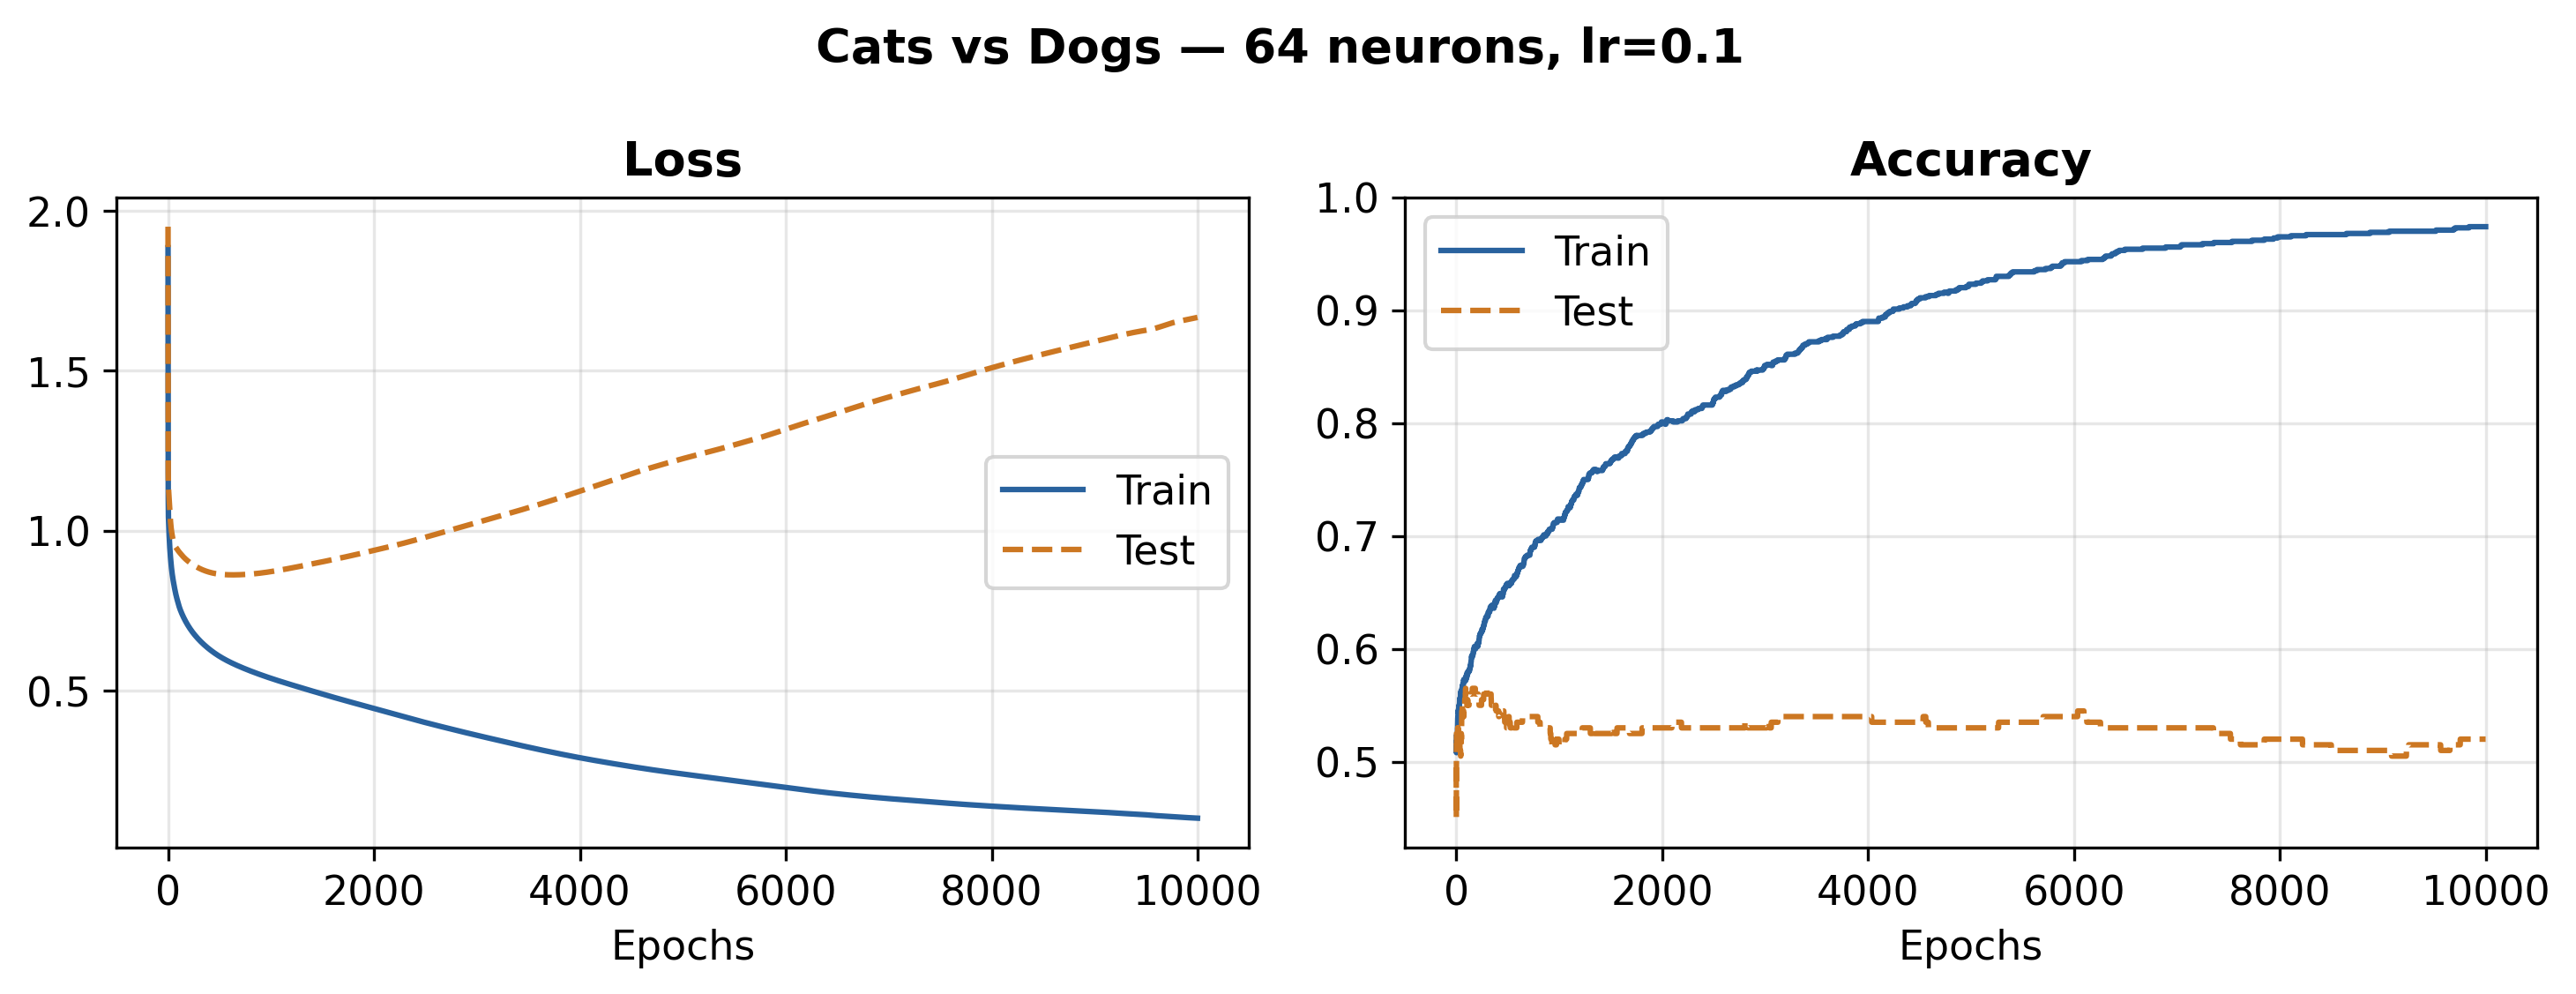
\includegraphics[width=0.92\textwidth]{images/overfitting_curves.png}
    \caption{Train vs test performance on cats vs dogs. The training curves look great --- but the test curves tell a different story. This is \textbf{overfitting}.}
\end{figure}

\begin{itemize}
  \item Training loss keeps decreasing
  \item \textbf{Test loss starts increasing} after some point
  \item Training accuracy keeps climbing
  \item \textbf{Test accuracy plateaus} or even drops
\end{itemize}

\begin{warnbox}[title=Overfitting]
When a model performs well on training data but poorly on unseen data, it's \textbf{overfitting}.

The model isn't learning general patterns --- it's \textbf{memorizing} the training examples.

It's like studying for an exam by memorizing the answers instead of understanding the material.
\end{warnbox}

Why does this happen?

\begin{enumerate}
  \item \textbf{Too many parameters, too little data.}
  Our network with 64 hidden neurons has $4096 \times 64 + 64 + 64 \times 1 + 1 = 262{,}273$ parameters.
  But we only have 1000 training images.

  \item \textbf{No regularization.}
  We haven't told the network to prefer simple solutions.

  \item \textbf{No data augmentation.}
  We haven't artificially increased the training set size.
\end{enumerate}

\begin{insightbox}[title=The Million-Dollar Question]
When your model underperforms, ask yourself:

\begin{quote}
\textbf{``Is this a problem with the data, the model, or the training?''}
\end{quote}

Here, the answer is clear: not enough data for this many parameters.

A data scientist's job isn't just to build models --- it's to \textbf{diagnose} why they fail and \textbf{decide} what to fix.
\end{insightbox}

This is as far as our two-layer network can take us on this dataset.

But it's not a failure. It's a \textbf{lesson}.

%% ============================================================
%% SECTION 12 — CONCLUSION
%% ============================================================
\section{What You've Built}

Stop.

Before we move on --- take a breath.

You started this series not knowing what a gradient was.
Now you've just coded a neural network that classifies images of cats and dogs.

\textit{From scratch. Without a framework. Without anyone telling you what to copy-paste.}

That's not nothing. That's rare.

Starting from nothing but a set of equations, you built:

\begin{resultbox}[title=Your Neural Network --- From Scratch]
\begin{enumerate}[label=\textbf{\arabic*.}]
  \item \textbf{Initialization} --- random parameters, controlled dimensions
  \item \textbf{Forward propagation} --- input to prediction in two matrix operations
  \item \textbf{Cost function} --- log-loss to measure errors
  \item \textbf{Backpropagation} --- six lines of gradient computation
  \item \textbf{Update} --- four subtractions (gradient descent)
  \item \textbf{Training loop} --- forward $\to$ cost $\to$ backward $\to$ update, repeat
  \item \textbf{Prediction} --- threshold at 0.5
  \item \textbf{Visualization} --- decision boundary plots
\end{enumerate}
\end{resultbox}

That's a complete neural network.

No framework. No library hiding the math. Just NumPy and understanding.

You tested it on toy data and got near-perfect classification.
You tested it on real images and discovered overfitting.
Both results matter.

\begin{quote}
\textit{Understanding why something fails is just as important as making it work.}
\end{quote}

\section{What's Next}

Right now, our network has exactly two layers. We chose 32 neurons. We chose sigmoid activation.

But what if we wanted \textbf{three layers}? Or five? Or fifty?

\begin{actionbox}[title=Next Stop --- Going Deeper]
What if we could build a network with \textbf{any number of layers}, \textbf{any number of neurons per layer}, and \textbf{any architecture we want}?

That's not a hypothetical. That's the next episode.

We'll generalize everything we've done to $L$ layers --- and you'll see that the code barely changes.

\textbf{Meet me in the next episode.}
\end{actionbox}

\vspace{2em}
\begin{center}
\rule{0.6\textwidth}{0.4pt}\\[1em]
{\small \textbf{Deep Learning From Scratch}}\\[0.3em]
{\small An open-source learning journey.}\\[0.8em]
{\small \textbf{GitHub:} \url{https://github.com/Pchambet/Deep-Learning-from-Scratch}}\\[0.3em]
{\small \textbf{LinkedIn:} \url{https://www.linkedin.com/in/pierre-chambet/}}\\[1em]
{\footnotesize \textcopyright\ 2026 Pierre Chambet}
\end{center}

\end{document}
